\documentclass[11pt,a4paper]{article}

\usepackage[margin=1in]{geometry}
\usepackage{mathptmx}
\usepackage{amsmath}
\usepackage{amssymb}
\usepackage{amsthm}
\usepackage{braket}
\usepackage{tikz}
\usepackage{quantikz}
\usepackage{enumitem}
\usepackage{hyperref}
\usepackage{xcolor}

\definecolor{circuitblue}{RGB}{40,80,160}

\hypersetup{
    colorlinks=true,
    linkcolor=circuitblue,
    urlcolor=circuitblue,
    citecolor=circuitblue
}

\theoremstyle{definition}
\newtheorem{definition}{Definition}[section]
\newtheorem{example}{Example}[section]

\theoremstyle{remark}
\newtheorem*{intuition}{Intuition}
\newtheorem*{keypoint}{Key Point}

\pagestyle{plain}

\setlength{\parindent}{0pt}
\setlength{\parskip}{6pt}

\begin{document}

\begin{center}
    {\LARGE \textbf{Parameterized Quantum Circuits}}\\[8pt]
    {\large QML}\\[12pt]
    \hrule
\end{center}

\vspace{12pt}
\tableofcontents
\newpage

%% ========================================================
\section{What Are Parameterized Quantum Circuits?}
%% ========================================================

\begin{definition}
a \textbf{parameterized quantum circuit} (PQC), also called a \textbf{variational ansatz}, is a quantum circuit containing gates with tunable parameters $\theta = (\theta_1, \theta_2, \ldots, \theta_p)$:
\[
U(\theta) = U_L(\theta_L) \cdot U_{L-1}(\theta_{L-1}) \cdots U_1(\theta_1)
\]
the circuit produces a parameterized quantum state $\ket{\psi(\theta)} = U(\theta)\ket{0}^{\otimes n}$ and the output is typically an expectation value:
\[
\boxed{f(\theta) = \bra{0}^{\otimes n} U^\dagger(\theta) \, O \, U(\theta) \ket{0}^{\otimes n} = \langle O \rangle_\theta}
\]
where $O$ is some observable (e.g., a pauli operator).
\end{definition}

PQCs r the workhorses of NISQ quantum computing. they r used in VQE, QAOA, quantum classifiers, quantum generative models --- basically everything.

\begin{keypoint}
the analogy to classical ML:
\begin{center}
\begin{tabular}{l|l}
\textbf{classical NN} & \textbf{PQC} \\
\hline
weights and biases $\theta$ & rotation angles $\theta$ \\
linear layer + activation & parameterized gates + entangling gates \\
forward pass & circuit execution \\
backprop & parameter shift rule \\
ReLU, sigmoid & measurement (born rule) \\
hidden layers & circuit layers (depth) \\
width (neurons per layer) & qubits
\end{tabular}
\end{center}
\end{keypoint}

%% ========================================================
\section{Single Qubit Rotation Gates}
%% ========================================================

the building blocks of PQCs r single-qubit rotation gates. these r the parameterized gates that get optimized during training.

\subsection{$R_x(\theta)$ --- Rotation Around X-Axis}

\[
R_x(\theta) = e^{-i\theta X/2} = \begin{pmatrix} \cos\frac{\theta}{2} & -i\sin\frac{\theta}{2} \\ -i\sin\frac{\theta}{2} & \cos\frac{\theta}{2} \end{pmatrix}
\]

\begin{center}
\begin{quantikz}
\lstick{$\ket{\psi}$} & \gate{R_x(\theta)} & \qw
\end{quantikz}
\end{center}

effect on the bloch sphere: rotation by angle $\theta$ around the x-axis.

special cases: $R_x(0) = I$, $R_x(\pi) = -iX$, $R_x(2\pi) = -I$.

\subsection{$R_y(\theta)$ --- Rotation Around Y-Axis}

\[
R_y(\theta) = e^{-i\theta Y/2} = \begin{pmatrix} \cos\frac{\theta}{2} & -\sin\frac{\theta}{2} \\ \sin\frac{\theta}{2} & \cos\frac{\theta}{2} \end{pmatrix}
\]

$R_y$ is special bcs its matrix entries r \textbf{real}. this means $R_y$ can create any real superposition: $R_y(\theta)\ket{0} = \cos(\theta/2)\ket{0} + \sin(\theta/2)\ket{1}$.

\subsection{$R_z(\theta)$ --- Rotation Around Z-Axis}

\[
R_z(\theta) = e^{-i\theta Z/2} = \begin{pmatrix} e^{-i\theta/2} & 0 \\ 0 & e^{i\theta/2} \end{pmatrix}
\]

$R_z$ only changes the relative phase between $\ket{0}$ and $\ket{1}$. it doesnt change the measurement probabilities in the computational basis.

\subsection{General Single-Qubit Rotation}

any single-qubit unitary can be decomposed as:
\[
U(\alpha, \beta, \gamma, \delta) = e^{i\alpha} R_z(\beta) R_y(\gamma) R_z(\delta)
\]

so 3 parameters (ignoring global phase) suffice for any single-qubit gate. in PQCs, we typically use combinations of $R_y$ and $R_z$ (or $R_x$ and $R_z$) to parameterize single-qubit operations.

\begin{example}
a common single-qubit variational layer:
\begin{center}
\begin{quantikz}
\lstick{$\ket{0}$} & \gate{R_y(\theta_1)} & \gate{R_z(\theta_2)} & \qw
\end{quantikz}
\end{center}
this can produce any state on the bloch sphere (2 parameters for 2 degrees of freedom).
\end{example}

%% ========================================================
\section{Ansatz Design}
%% ========================================================

\subsection{What is an Ansatz?}

\begin{definition}
an \textbf{ansatz} is the specific circuit architecture u choose for ur PQC. it defines:
\begin{enumerate}
    \item which parameterized gates to use
    \item how to arrange them (layer structure)
    \item which qubits to entangle and how
    \item the total number of parameters
\end{enumerate}
the choice of ansatz determines the hypothesis class of ur quantum model.
\end{definition}

\subsection{Hardware-Efficient Ansatz (HEA)}

\begin{definition}
a \textbf{hardware-efficient ansatz} is designed to match the native gate set and connectivity of a specific quantum processor. layers alternate between single-qubit rotations and entangling gates native to the hardware.
\end{definition}

\begin{center}
\begin{quantikz}
\lstick{$q_0$} & \gate{R_y(\theta_1)} & \gate{R_z(\theta_2)} & \ctrl{1} & \gate{R_y(\theta_7)} & \gate{R_z(\theta_8)} & \ctrl{1} & \qw \\
\lstick{$q_1$} & \gate{R_y(\theta_3)} & \gate{R_z(\theta_4)} & \targ{} & \gate{R_y(\theta_9)} & \gate{R_z(\theta_{10})} & \targ{} & \qw \\
\lstick{$q_2$} & \gate{R_y(\theta_5)} & \gate{R_z(\theta_6)} & \qw & \gate{R_y(\theta_{11})} & \gate{R_z(\theta_{12})} & \qw & \qw
\end{quantikz}
\end{center}

each ``layer'' consists of:
\begin{enumerate}
    \item single-qubit rotations on every qubit ($R_y, R_z$)
    \item entangling gates between connected qubit pairs (CNOT, CZ)
\end{enumerate}

repeat for $L$ layers. total parameters: $\sim 2nL$ (for $n$ qubits).

\begin{keypoint}
HEA pros:
\begin{itemize}
    \item low circuit depth (native gates, no compilation overhead)
    \item matches hardware connectivity (no SWAP gates needed)
    \item simple to implement
\end{itemize}
HEA cons:
\begin{itemize}
    \item no problem structure encoded --- the ansatz doesnt ``know'' anything about ur task
    \item prone to barren plateaus (random-looking circuits at initialization)
    \item may need many layers to be expressive enough
\end{itemize}
\end{keypoint}

\subsection{Problem-Inspired Ansatze}

\begin{definition}
a \textbf{problem-inspired ansatz} uses domain knowledge to design the circuit. examples:
\begin{itemize}
    \item \textbf{UCCSD} (unitary coupled cluster): for quantum chemistry. encodes the structure of electron excitations
    \item \textbf{QAOA}: for combinatorial optimization. alternates between problem and mixer hamiltonians
    \item \textbf{Hamiltonian variational ansatz}: uses trotterized time evolution under the problem hamiltonian
\end{itemize}
\end{definition}

\begin{intuition}
problem-inspired ansatze trade generality for efficiency. by encoding problem structure, they can reach good solutions with fewer parameters and shallower circuits. the downside is u need to know smtg abt ur problem to design the ansatz. for QML, this means choosing the right data encoding and circuit structure for ur specific classification or regression task.
\end{intuition}

\subsection{Entangling Patterns}

the entangling structure significantly affects the circuit's expressive power:

\textbf{linear entanglement}: each qubit entangles with its neighbor.
\begin{center}
\begin{quantikz}
& \ctrl{1} & \qw & \qw & \qw \\
& \targ{} & \ctrl{1} & \qw & \qw \\
& \qw & \targ{} & \ctrl{1} & \qw \\
& \qw & \qw & \targ{} & \qw
\end{quantikz}
\end{center}

\textbf{circular entanglement}: same as linear but with an additional gate connecting the last qubit to the first.

\textbf{full (all-to-all) entanglement}: every pair of qubits gets an entangling gate.
\begin{center}
\begin{quantikz}
& \ctrl{1} & \ctrl{2} & \ctrl{3} & \qw \\
& \targ{} & \qw & \qw & \qw \\
& \qw & \targ{} & \qw & \qw \\
& \qw & \qw & \targ{} & \qw
\end{quantikz}
\end{center}

\begin{keypoint}
more entanglement $=$ more expressiveness but also more noise and potentially more barren plateaus. the sweet spot depends on the problem and the hardware.
\end{keypoint}

%% ========================================================
\section{Expressibility of PQCs}
%% ========================================================

\subsection{What Does Expressibility Mean?}

\begin{definition}
the \textbf{expressibility} of a PQC measures how well the circuit can explore the full hilbert space. a highly expressible circuit can produce states close to any target state. mathematically, its quantified by how close the distribution of output states is to the uniform (Haar random) distribution over unitaries.
\end{definition}

sim, johnson, and aspuru-guzik (2019) introduced a quantitative measure:

\[
\text{Expr} = D_{\text{KL}}\left(\hat{P}_{\text{PQC}}(F) \,\|\, P_{\text{Haar}}(F)\right)
\]

where $F = |\braket{\psi|\phi}|^2$ is the fidelity between pairs of randomly parameterized states, $\hat{P}_{\text{PQC}}$ is the distribution from the PQC, and $P_{\text{Haar}}$ is the distribution from Haar random unitaries.

low expressibility value $=$ the PQC covers the hilbert space well $=$ good.

\begin{example}
expressibility hierarchy (from their paper):
\begin{itemize}
    \item single $R_y$ layer, no entanglement: low expressibility (restricted to real product states)
    \item $R_y + R_z$ layers with CNOT entanglement: moderate expressibility
    \item multiple layers of $R_y + R_z + $ CNOT: high expressibility (approaches Haar random)
    \item too few parameters or wrong topology: low expressibility regardless of depth
\end{itemize}
\end{example}

\subsection{Entangling Capability}

\begin{definition}
the \textbf{entangling capability} of a PQC measures how much entanglement the circuit can generate, averaged over random parameter values. typically measured using the meyer-wallach entanglement measure:
\[
Q = \frac{2}{n}\sum_{j=1}^n \left(1 - \text{tr}(\rho_j^2)\right)
\]
where $\rho_j$ is the reduced density matrix of qubit $j$. $Q = 0$ for product states, $Q \to 1$ for highly entangled states.
\end{definition}

\begin{keypoint}
expressibility and entangling capability r related but distinct:
\begin{itemize}
    \item u can have a highly expressible circuit with low entangling capability (e.g., many single-qubit gates, no entanglement)
    \item u need BOTH expressibility AND entangling capability for powerful QML models
    \item but too much of either can lead to trainability issues (barren plateaus)
\end{itemize}
\end{keypoint}

%% ========================================================
\section{Circuit Depth vs Expressibility Tradeoff}
%% ========================================================

\begin{center}
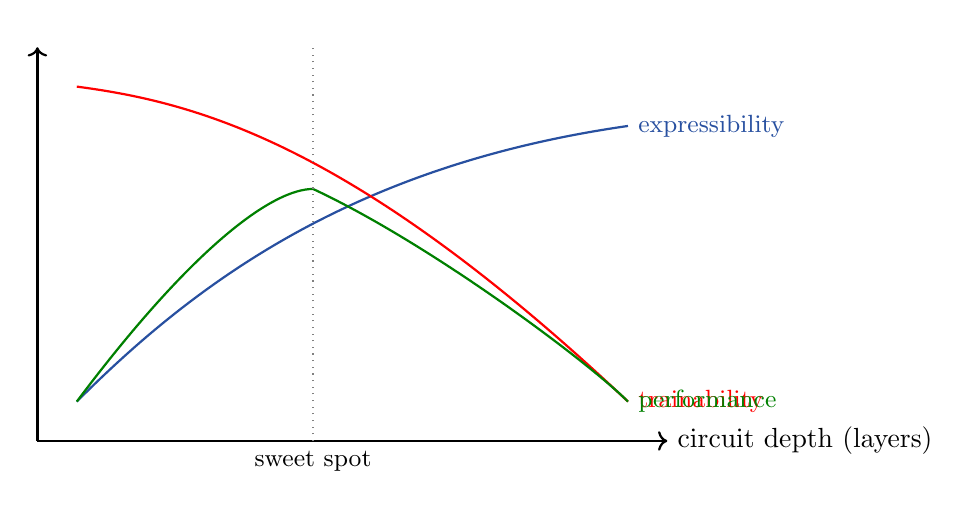
\begin{tikzpicture}[scale=1]
    \draw[->, thick] (0,0) -- (8,0) node[right] {circuit depth (layers)};
    \draw[->, thick] (0,0) -- (0,5) node[above] {};

    \draw[thick, circuitblue] (0.5,0.5) .. controls (2,2) and (4,3.5) .. (7.5,4) node[right, font=\small] {expressibility};
    \draw[thick, red] (0.5,4.5) .. controls (2,4.3) and (4,3.8) .. (7.5,0.5) node[right, font=\small] {trainability};
    \draw[thick, green!50!black] (0.5,0.5) .. controls (2,2.5) and (3,3.2) .. (3.5,3.2) .. controls (5,2.5) and (7,1) .. (7.5,0.5) node[right, font=\small] {performance};

    \draw[dotted, gray] (3.5,0) -- (3.5,5);
    \node[below, font=\small] at (3.5,0) {sweet spot};
\end{tikzpicture}
\end{center}

\begin{keypoint}
the depth dilemma:
\begin{itemize}
    \item \textbf{too shallow}: not expressive enough. the model cant represent the target function. underfitting.
    \item \textbf{too deep}: hits barren plateaus (gradients vanish exponentially). also more noise. cant train even if the model is expressive enough.
    \item \textbf{sweet spot}: enough depth for the task but not so much that training breaks. typically 5--20 layers for current QML tasks.
\end{itemize}
finding this sweet spot is one of the open challenges in QML.
\end{keypoint}

%% ========================================================
\section{Data Encoding Circuits}
%% ========================================================

in QML, PQCs have two types of parameters:
\begin{enumerate}
    \item \textbf{data parameters}: encoding the classical input $x$ into the quantum state (the ``feature map'')
    \item \textbf{trainable parameters}: angles that r optimized during training
\end{enumerate}

\subsection{Encoding Strategies}

\textbf{basis encoding}: encode $x$ as a computational basis state.
\[
x = 5 = 101_2 \quad \to \quad \ket{101}
\]
simple but limited. needs $n = \lceil\log_2 N\rceil$ qubits for $N$ data points.

\textbf{amplitude encoding}: encode the data vector as amplitudes of a quantum state.
\[
\vec{x} = (x_1, \ldots, x_N) \quad \to \quad \ket{\psi_x} = \frac{1}{\|\vec{x}\|}\sum_{i=1}^N x_i \ket{i}
\]
exponentially compact ($\log N$ qubits for $N$-dimensional data) but hard to prepare efficiently.

\textbf{angle encoding}: encode each feature as a rotation angle.
\[
\ket{\psi_x} = \bigotimes_{i=1}^n R_y(x_i)\ket{0}
\]

\begin{center}
\begin{quantikz}
\lstick{$\ket{0}$} & \gate{R_y(x_1)} & \qw \\
\lstick{$\ket{0}$} & \gate{R_y(x_2)} & \qw \\
\lstick{$\ket{0}$} & \gate{R_y(x_3)} & \qw
\end{quantikz}
\end{center}

simple and efficient. but product states --- no entanglement. limited expressiveness.

\textbf{IQP (instantaneous quantum polynomial) encoding}: uses $Z$-rotations and entangling gates.
\[
U(x) = \exp\left(i\sum_{j}x_j Z_j + i\sum_{j<k} x_j x_k Z_j Z_k\right)
\]

this creates entanglement between features and r used in the havlicek et al. (2019) quantum kernel classifier.

\textbf{data re-uploading}: encode data \textbf{multiple times} throughout the circuit, interleaved with trainable gates.

\begin{center}
\begin{quantikz}
\lstick{$\ket{0}$} & \gate{R_y(x)} & \gate{R_z(\theta_1)} & \gate{R_y(x)} & \gate{R_z(\theta_2)} & \gate{R_y(x)} & \gate{R_z(\theta_3)} & \meter{}
\end{quantikz}
\end{center}

\begin{keypoint}
perez-salinas et al. (2020) showed that data re-uploading with a single qubit is a \textbf{universal quantum classifier}. by encoding data multiple times, each layer can implement increasingly complex nonlinear functions of the input. this is analogous to how depth in classical neural networks increases function complexity.

the function computed by a data re-uploading circuit with $L$ layers is a partial fourier series with frequencies up to $L$:
\[
f(x) = \sum_{k=-L}^{L} c_k e^{ikx}
\]
more layers $=$ higher frequencies $=$ more complex decision boundaries.
\end{keypoint}

\subsection{Data Encoding Comparison}

\begin{center}
\begin{tabular}{l|c|c|c}
encoding & qubits for $d$ features & circuit depth & expressiveness \\
\hline
basis & $\lceil\log_2 d\rceil$ & $O(d)$ & limited \\
amplitude & $\lceil\log_2 d\rceil$ & $O(d)$ & limited \\
angle & $d$ & $O(1)$ per feature & moderate \\
IQP & $d$ & $O(d)$ & high \\
re-uploading & $\geq 1$ & $O(Ld)$ & universal
\end{tabular}
\end{center}

%% ========================================================
\section{The Full Variational Circuit}
%% ========================================================

a typical variational QML circuit combines data encoding and trainable layers:

\begin{center}
\begin{quantikz}
\lstick{$\ket{0}$} & \gate[3]{S(x)} & \gate[3]{W(\theta_1)} & \gate[3]{S(x)} & \gate[3]{W(\theta_2)} & \meter{} \\
\lstick{$\ket{0}$} & & & & & \meter{} \\
\lstick{$\ket{0}$} & & & & & \meter{}
\end{quantikz}
\end{center}

where $S(x)$ is the data encoding circuit and $W(\theta)$ is the trainable variational layer.

the full circuit is:
\[
U(\theta, x) = W(\theta_L) S(x) W(\theta_{L-1}) S(x) \cdots W(\theta_1) S(x)
\]

and the model output is:
\[
f(\theta, x) = \text{tr}\left(O \cdot U(\theta, x)\ket{0}\bra{0}U^\dagger(\theta, x)\right)
\]

\begin{keypoint}
the structure matters enormously:
\begin{itemize}
    \item wt data encoding $S(x)$ u use determines the quantum feature space
    \item wt trainable circuit $W(\theta)$ u use determines wt functions u can learn within that feature space
    \item the number of re-uploads of the data determines the frequency spectrum of the model
    \item the entanglement structure determines correlations between features
\end{itemize}
this is not just hyperparameter tuning --- the circuit architecture fundamentally determines wt the model can and cannot learn.
\end{keypoint}

%% ========================================================
\section{Gradient Computation: The Parameter Shift Rule}
%% ========================================================

\subsection{The Problem}

to train a PQC, we need gradients $\frac{\partial f}{\partial \theta_i}$. but we cant do backprop on a quantum circuit (no intermediate states r accessible). the solution: the \textbf{parameter shift rule}.

\subsection{Derivation}

\begin{definition}
for a gate of the form $G(\theta) = e^{-i\theta P/2}$ where $P$ is a pauli operator ($P^2 = I$), the gradient is:
\[
\boxed{\frac{\partial}{\partial \theta}\langle O \rangle_\theta = \frac{\langle O \rangle_{\theta + \pi/2} - \langle O \rangle_{\theta - \pi/2}}{2}}
\]
\end{definition}

\textbf{derivation}: the expectation value is:
\[
\langle O \rangle_\theta = \bra{0} U^\dagger_{-}(\theta) \, G^\dagger(\theta) \, U^\dagger_{+} \, O \, U_{+} \, G(\theta) \, U_{-}(\theta) \ket{0}
\]

where $U_+$ and $U_-$ are the circuit parts after and before the gate $G(\theta)$.

using $G(\theta) = \cos(\theta/2)I - i\sin(\theta/2)P$ and differentiating:
\begin{align}
\frac{\partial G}{\partial \theta} &= -\frac{1}{2}\sin(\theta/2)I - \frac{i}{2}\cos(\theta/2)P \\
&= -\frac{i}{2}P \cdot G(\theta) = \frac{1}{2}(G(\theta + \pi/2) - G(\theta - \pi/2)) \cdot (\text{using } e^{-iP\pi/4})
\end{align}

after working through the algebra:
\[
\frac{\partial \langle O \rangle}{\partial \theta} = \frac{1}{2}\left(\langle O \rangle_{\theta + \pi/2} - \langle O \rangle_{\theta - \pi/2}\right)
\]

\begin{keypoint}
the parameter shift rule is beautiful bcs:
\begin{itemize}
    \item it gives the \textbf{exact} gradient (not an approximation like finite differences)
    \item it only requires 2 circuit evaluations per parameter
    \item it works on real quantum hardware (no need for intermediate state access)
    \item total cost for all $p$ gradients: $2p$ circuit evaluations
    \item this is worse than classical backprop ($O(1)$ overhead) but much better than finite differences ($O(p)$ with approximation error)
\end{itemize}
\end{keypoint}

\begin{example}
compute $\frac{\partial}{\partial \theta} \langle Z \rangle$ for the circuit $R_y(\theta)\ket{0}$:

$\langle Z \rangle_\theta = \cos\theta$

parameter shift: $\frac{1}{2}(\cos(\theta + \pi/2) - \cos(\theta - \pi/2)) = \frac{1}{2}(-\sin\theta - \sin\theta) = -\sin\theta$

direct differentiation: $\frac{d}{d\theta}\cos\theta = -\sin\theta$. $\checkmark$
\end{example}

\subsection{Gradient-Free Methods}

alternatives to gradient-based optimization:

\begin{itemize}
    \item \textbf{COBYLA}: constrained optimization by linear approximation. no gradients needed.
    \item \textbf{SPSA} (simultaneous perturbation stochastic approximation): estimate the gradient with only 2 circuit evaluations total (independent of $p$). noisy but cheap.
    \item \textbf{Nelder-Mead}: simplex method. good for low-dimensional optimization.
    \item \textbf{Bayesian optimization}: builds a surrogate model of the loss landscape. good for expensive evaluations.
\end{itemize}

\begin{keypoint}
in practice, the choice between gradient-based and gradient-free optimization depends on:
\begin{itemize}
    \item number of parameters (gradient-free methods dont scale well beyond $\sim 50$--$100$ parameters)
    \item noise level (noisy gradients may make gradient-free methods preferable)
    \item circuit evaluation cost (if each circuit run is expensive, SPSA with 2 evaluations per step is attractive)
    \item the loss landscape (if its very noisy or has many local minima, gradient-free methods may navigate better)
\end{itemize}
\end{keypoint}

%% ========================================================
\section{Common PQC Architectures for QML}
%% ========================================================

\subsection{Circuit 1: RealAmplitudes}

\begin{center}
\begin{quantikz}
\lstick{$q_0$} & \gate{R_y(\theta_1)} & \ctrl{1} & \gate{R_y(\theta_4)} & \ctrl{1} & \qw \\
\lstick{$q_1$} & \gate{R_y(\theta_2)} & \targ{} & \gate{R_y(\theta_5)} & \targ{} & \qw \\
\lstick{$q_2$} & \gate{R_y(\theta_3)} & \qw & \gate{R_y(\theta_6)} & \qw & \qw
\end{quantikz}
\end{center}

only $R_y$ rotations (real amplitudes) with linear CNOT entanglement. simple, low parameter count, easy to train.

\subsection{Circuit 2: EfficientSU2}

\begin{center}
\begin{quantikz}
\lstick{$q_0$} & \gate{R_y(\theta_1)} & \gate{R_z(\theta_4)} & \ctrl{1} & \gate{R_y(\theta_7)} & \gate{R_z(\theta_{10})} & \qw \\
\lstick{$q_1$} & \gate{R_y(\theta_2)} & \gate{R_z(\theta_5)} & \targ{} & \gate{R_y(\theta_8)} & \gate{R_z(\theta_{11})} & \qw \\
\lstick{$q_2$} & \gate{R_y(\theta_3)} & \gate{R_z(\theta_6)} & \qw & \gate{R_y(\theta_9)} & \gate{R_z(\theta_{12})} & \qw
\end{quantikz}
\end{center}

$R_y + R_z$ rotations (full SU(2) on each qubit) with entanglement. more expressive than RealAmplitudes.

\subsection{Circuit 3: TwoLocal}

a generalization where u can choose any rotation gates and any entanglement pattern. the qiskit \texttt{TwoLocal} class lets u specify both.

\subsection{Circuit 4: Data Re-uploading Classifier}

\begin{center}
\begin{quantikz}
\lstick{$\ket{0}$} & \gate{R_x(x_1)} & \gate{R_y(\theta_1)} & \gate{R_z(\theta_2)} & \gate{R_x(x_1)} & \gate{R_y(\theta_3)} & \gate{R_z(\theta_4)} & \meter{}
\end{quantikz}
\end{center}

single qubit, data encoded multiple times. universal for any number of features (with enough qubits and layers).

%% ========================================================
\section{The Function Space of PQCs}
%% ========================================================

\subsection{Fourier Analysis of PQC Outputs}

\begin{keypoint}
schuld, sweke, and meyer (2021) showed that the functions computed by PQCs r \textbf{partial fourier series}. specifically, for a PQC with data encoding gates $e^{-ix_j G_j}$ (where $G_j$ r generators with eigenvalues in a discrete set $\Lambda$), the output function is:
\[
f(x) = \sum_{\omega \in \Omega} c_\omega e^{i\omega x}
\]
where $\Omega$ is the set of accessible frequencies, determined by the eigenvalues of the generators and the number of times data is encoded.

key implications:
\begin{itemize}
    \item the \textbf{data encoding} determines which frequencies r available
    \item the \textbf{trainable parameters} determine the fourier coefficients $c_\omega$
    \item more data re-uploads $=$ higher frequencies $=$ more complex functions
    \item this gives a precise characterization of wt functions PQCs can and cannot learn
\end{itemize}
\end{keypoint}

\begin{example}
single qubit, $R_x(x)$ encoding, $L$ re-uploads:

accessible frequencies: $\omega \in \{-L, -L+1, \ldots, L-1, L\}$

the model can represent $2L + 1$ fourier components $\to$ functions with resolution $\sim 1/L$.
\end{example}

%% ========================================================
\section{Summary}
%% ========================================================

\begin{keypoint}
PQCs in a nutshell:
\begin{enumerate}
    \item PQCs r quantum circuits with tunable parameters --- the quantum analogue of neural networks
    \item rotation gates ($R_x, R_y, R_z$) provide the parameterization
    \item ansatz design (hardware-efficient vs problem-inspired) determines the hypothesis class
    \item expressibility measures how well the ansatz covers the hilbert space
    \item data encoding (angle, amplitude, IQP, re-uploading) determines the quantum feature space
    \item the parameter shift rule gives exact gradients with $2p$ circuit evaluations
    \item PQC outputs r partial fourier series --- the encoding determines frequencies, the trainable parameters determine coefficients
    \item the sweet spot between expressibility and trainability is the central design challenge
\end{enumerate}
next: QAOA --- the first major application of PQCs to combinatorial optimization, and a stepping stone to quantum classifiers.
\end{keypoint}

\end{document}
